\documentclass{article}
\usepackage[utf8]{inputenc}
\usepackage{amsmath}
\usepackage{listings}
\usepackage{geometry}
\usepackage{graphicx}
\usepackage{subfig}
\usepackage{gensymb}
\usepackage{cancel}
\usepackage{physics}
\usepackage[colorlinks=true]{hyperref}
\title{%
Project 4 - Phase Transitions in Magnetic Systems \\
\Large A study using Montecarlo Cycles to simulate \\
\Large and observe phase transitions in \\
\Large magnetic systems of various sizes \\
\large FYS3150 at University of Oslo}
\author{Simen Løken}
\date{November 2020}
\footskip = 90pt
\topmargin = -40pt

\begin{document}
\nocite{projtext}
\maketitle
\tableofcontents
\section{Abstract}
In this report, we'll introduce an Ising Model from the ground up using the Metropolis algorithm and get to understand it better through testing and prodding. After sufficiently examining the Ising Model at a basic level, we will then expand our model in order to determine the Curie Temperature $T_C$ numerically. Additionally, we aim to explore the properties of ferromagnetic materials in a range around $T_C$, and looking at various behaviours.
\section{Introduction}
The \textbf{Ising Model}, named after Ernst Ising, is a model for studying the magnetic properties of ferromagnetic materials. For simplicity's sake, the model is simplified to only allow for a given spin to interact with it's neighbouring spins, but can still be used to illustrate many different important properties in magnetism. \newline
We're going to be doing this by employing the \textbf{Metropolis algorithm}, using \textbf{Monte Carlo cycles}. The reason for this is that a pure numerical to a Ising Model on it's own would be exceptionally intensive to calculate, even impossible in some cases. \newline
The Metropolis algorithm allows us to find the probability distribution function of extensive, complicated systems, saving precious computation time without sacrificing the integrity of our results. 
\newline
As previously stated, the primary reason for us using the Ising Model is it's applicability to the real world with exceptionally good results, being one of the few fully solvable models for computing thermodynamic quantities. This in turn allows us to study magnetism, and it's properties and interpret them at a sufficiently microscopic level.
\newline
In this report, we're going to be constructing such an algorithm for solving a two dimensional Ising Model using the Metropolis algorithm. Firstly, we're going to be comparing our numerical results for a $2\times2$ lattice to it's analytical counterpart, then expanding on the size of our model to find the number of Monte Carlo sweeps required to reach an equilibrium for different initial conditions, like lattice size or temperature. This will serve as a good indicator for how many calculations we will need to perform in order to find good solutions that corrolate with reality.\newline
From there, we will then let our model run continuously for an increasing temperature so we can properly study the phase transition of a magnetic system given by it's specific heat, and then extracting that information to find Curie Temperature $T_C$, the temperature where a material loses it's magnetic properties. Following this, we can compare our numerical Curie Temperature against the analytical solution, first derived by Lars Onsager\cite{lars} to be $T_C \approx 2.269$ \newpage
\section{Theory and Method}
\subsection{The Partition Function}
I mentioned in the introduction that for the Ising Model, we're only examining the neighbouring spins. This has a couple of effects on our model. Primarily, and most importantly, for a 2D model, it tells us that any given $\Delta E$, that is, change of energy in a given time step, can only be one of five distinct values. To further illustrate this, take a look at this figure:
\begin{figure}[ht!]
    \centering
    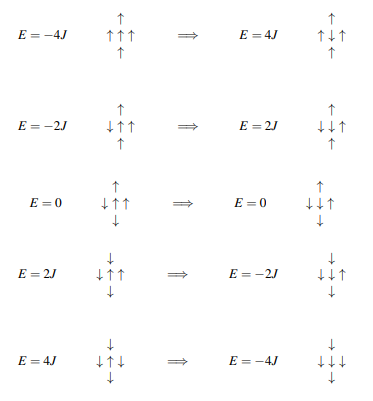
\includegraphics[scale=0.8]{energies.png}
    \caption{All possible different configurations of neighbouring spins in relation to the spin of the "observer"\newline
    Notice that, for any given orientation of our observer spin, there are only five possible neighbouring configurations, and that they mirror each other for different orientations of our observer.
    \newline Illustration: \cite{lecnotes}}
    \label{figEn}
\end{figure}
This is very useful, as it means we can predict, or rather, calculate all possible energies ahead of time, saving precious computational power in an already pretty heavy computation. \newline
The corresponding partition function would then be given as:
\begin{equation}
    Z = \sum_s e^{\frac{-E_s}{k_B T}}
\end{equation}
where $s$ is a given state, $E_s$ is the energy of the state $s$, $k_B$ is the Boltzmann constant and $T$ is the temperature. From now on, this denominator will be referred to as $\beta$, such that $\beta = \frac{1}{k_B T}$.
\newline Subsequently, the Boltzmann distribution of our system becomes:
\begin{equation}
    P(E_i) = \frac{e^{-\beta E_i}}{Z} = \frac{e^{-\beta E_i}}{\sum_s e^{-\beta E_s}}
\end{equation}
\subsection{Boundary Conditions}
But what about the fringe case where our observer spin does not have four neighbouring spins. In the case of our observer being on the edge of the lattice, it'd only have three, and if it were in the corner only two! \newline
There are several ways to remedy this. You could for example, every time an observer is chosen, check it's corresponding $x$ and $y$ values. If any of those were either 0 or $L$ (for a $L\times L$ lattice), you could fix it accordingly. Alternatively, we could instead assume our lattice to be continuous, that is, if our observer is on the left-most side at some height $y$, then we'd assume it's left neighbour to be the right-most spin at height $y$.
\subsection{Analytical Values} \label{anal}
We can also derive the values we're calculating analytically. Most importantly, the expectation value for $E$ and $M$ is given as:
\begin{equation}
    \langle E \rangle = \frac{1}{Z} \sum_i^{N-1} E_i e^{-\beta E_i}
\end{equation}
\begin{equation} \label{m}
    \langle M \rangle = \frac{1}{Z} \sum_i^{N-1} M_i e^{-\beta E_i}
\end{equation}
Consequently, their squares can be calculated as:
\begin{equation}
    \langle E^2 \rangle = \frac{1}{Z} \sum_i^{N-1} (E_i e^{-\beta E_i})^2
\end{equation}
\begin{equation}
    \langle M^2 \rangle = \frac{1}{Z} \sum_i^{N-1} (M_i e^{-\beta E_i})^2
\end{equation}
We can then proceed to use these calculations for the rest of our analytical values, namely the specific heat, or heat capacity, $C_V$, given as:
\begin{equation}
    C_V = \frac{\langle E^2 \rangle - \langle E \rangle^2}{k_B T^2}
\end{equation}
The numerator of this equation is otherwise known as the variance of $E$.\newline
Additionally, using the same principle, the magnetic susceptibility $\chi$ can be expressed as:
\begin{equation}
    \chi = \frac{\langle M^2 \rangle - \langle M \rangle^2}{k_B T}
\end{equation}
A full derivation of the analytical values for $L = 2$ can be found in appendix A.
\newpage
\subsection{The Theory of Phase Transitions}
Additionally, we'll have to define some properties of physical quantities close to the Curie Temperature, in order to enable us extracting the numerical Curie Temperature as alluded to in the introduction. \newline
For the Ising Model, we can assume it's physical quantities abide by power law behavior, and thusly the mean magnetization is given by:
\begin{equation*}
    \lange M(T)\rangle \sim (T - T_C)^\beta
\end{equation*}
where $\beta$ is the critical exponent, given as $\beta = \frac{1}{8}$.
\newline
Following the same principal, we can describe the heat capacity $C_V$ and magnetic susceptibility $\chi$ as:
\begin{equation*}
    C_V(T) \sim |T_C - T|^\alpha
\end{equation*}
\begin{equation*}
    \chi(X) \sim |T_C - T|^\gamma
\end{equation*}
for $\alpha = 0$ and $\gamma = \frac{7}{4}$. \newline
Another consequence of treating these properties like so is that the correlation length, which is expected to in the order of the lattice spacing when $T \gg T_C$. As $T$ then approaches $T_C$, the spins become more correlated and the correlation length increases as we approach $T_C$. \newline
The divergent behavior can then be described as:
\begin{equation} \label{1}
    \xi(T) \sim |T_C - T|^v
\end{equation}
The phase transition is then characterized by its correlation length, which spans the entirety of the system. As our lattice is of a finite length $L$, $\xi$ will be proportional to $L$. If we then apply finite size scaling relations we can relate the behavior at finite lattices with results for an infinitely large lattice. The Curie Temperature then scales like so:
\begin{equation}
    T_C(L) - T_C(L=\infty) = aL^{\frac{-1}{v}}
\end{equation}
where $a$ is a constant and $v$ is defined through Equation [\ref{1}].
\newline
Following this assessment, we set assign $T = T_C$, giving the mean magnetization, heat capacity and magnetic susceptibility as:
\begin{equation*}
    \lange M(T)\rangle \sim (T - T_C)^\beta \xrightarrow{} L^{\frac{-\beta}{v}}
\end{equation*}
\begin{equation*}
    C_V(T) \sim |T_C - T|^\alpha \xrightarrow{} L^{\frac{\alpha}{v}}
\end{equation*}
\begin{equation*}
    \chi(X) \sim |T_C - T|^\gamma \xrightarrow{} L^{\frac{\gamma}{v}}
\end{equation*}
\newpage
\subsection{The Numerical Model} \label{algo}
Knowing everything we've discussed, we can now go through our model in it's entirety:
\begin{enumerate}
    \item Generate a set of spins in a lattice $L\times L$, either randomized or in a uniform configuration
    \item Calculate all possible values of $\Delta E$ ahead of time
    \item Retrieve initial conditions for $E$ and $M$ respectively. $M$ using the sum of the magnetic moment of our lattice and $E$ from summing energies in for all possible $x$ and $y$.
    \item Choose one random set of coordinates to be our observation and find its $\Delta E$
    \item Compare then a random number against our registered energy for $\Delta E$. If it is smaller or equal, then use this new $\Delta E$. If not, choose a new set of coordinates at step 4.
    \item If 6 was successful, then flip the spin of our current observer, and extract $M$ and $E$ given coordinates $x$, $y$ and energy $\Delta E$ respectively
    \item Go to 4
\end{enumerate}
Each run through of this algorithm is called a Monte Carlo cycle. After we are done with $N$ cycles, we can then divide our results by $N$ to normalize our results.
\newpage
\section{Results}
Let us first calibrate our algorithm by comparing it to it's analytical values. \newline We find:
\begin{figure}[ht!]
\centering
\subfloat[$\langle E \rangle$]{
  \includegraphics[width=65mm]{fig39.png}
}
\subfloat[$\langle M \rangle$]{
  \includegraphics[width=65mm]{fig40.png}
}
\newline
\subfloat[$C_V$]{
  \includegraphics[width=65mm]{fig41.png}
}
\subfloat[$\chi$]{
  \includegraphics[width=65mm]{fig42.png}
}
\caption{The stabilization as we increase the number of Monte Carlo cycles for temperature $T = 1$. We see that $10^4$ cycles is sufficient for a proper stabilization. \newline
\textbf{!NB!} I now noticed that for these plots and the subsequent ones looking at stabilization rates, the $x$-axis says Temperature. That is of course wrong, it should say number of cycles.}

\end{figure}
\newline
We see here clearly that it is sufficient for a lattice of dimension $2 \times 2$ to use $10^4$ Monte Carlo cycles. \newpage
Let us now expand our model to instead be a $20 \times 20$ lattice. Let us at the same time examine the effects of ordering our lattice:
\begin{figure}[ht!]
\centering
\subfloat[Ordered $\langle E \rangle$]{
  \includegraphics[width=65mm]{fig55.png}
}
\subfloat[Unordered $\langle E \rangle$]{
  \includegraphics[width=65mm]{fig47.png}
}
\newline
\subfloat[Ordered $\langle M \rangle$]{
  \includegraphics[width=65mm]{fig56.png}
}
\subfloat[Unordered $\langle M \rangle$]{
  \includegraphics[width=65mm]{fig48.png}
}
\caption{Here are the expectation values respectively for temperature $T = 1$ \newline
Note that all spins in the ordered variant were pointed up at initialization}
\end{figure} \newpage
We see here how the energy and magnetic expectation values change for ordered and unordered variants for a temperature below the Curie Temperature. Let us now examine a case where we are past the Curie Temperature, $T = 2.4$
\begin{figure}[ht!]
\centering
\subfloat[Ordered $\langle E \rangle$]{
  \includegraphics[width=65mm]{fig59.png}
}
\subfloat[Unordered $\langle E \rangle$]{
  \includegraphics[width=65mm]{fig51.png}
}
\newline
\subfloat[Ordered $\langle M \rangle$]{
  \includegraphics[width=65mm]{fig60.png}
}
\subfloat[Unordered $\langle M \rangle$]{
  \includegraphics[width=65mm]{fig52.png}
}
\caption{Here are the expectation values respectively for temperature $T = 2.4$ \newline
Note that all spins in the ordered variant were pointed up at initialization}
\end{figure} \newline
We see here the effects on a material that has a temperature past it's Curie Temperature $T_C$\newline
An interesting take away here is that, although they end up at the same result (within a margin of error) the start at opposite sides of their analytical value depending on whether or not the the initial state was ordered or not.
\newpage
Additionally, let us examine the accepted configurations. An accepted configuration is a configuration that passes part 5 of the algorithm described in Section [\ref{algo}]
\newline
\begin{figure}[ht!]
\centering
\subfloat[Accepted configs for $T = 1$]{ \label{1}
  \includegraphics[width=65mm]{fig29.png}
}
\subfloat[Accepted configs for $T = 2.4$]{ \label{2}
  \includegraphics[width=65mm]{fig34.png}
}
\caption{The number of accepted configs for each temperature respectively. \newline
For $T=1$, the function is logarithmic, dying off as we increase the number of cycles \newline
For $T=2.4$, the function is linear, increase linearly as we add more and more Monte Carlo sweeps}
\end{figure}
The main take away here is that the number of accepted configurations is close to constant for a $T$ past it's Curie Temperature, as opposed to a lower temperature, which has a logarithmic rate of accepted configurations.
\newline
Let us now examine the probability of a given energy for these two configurations.
\begin{figure}[ht!]
\centering
\subfloat[Probability of finding an energy for $T = 1$]{
  \includegraphics[width=65mm]{fig37.png}
}
\subfloat[Probability of finding an energy for $T = 2.4$]{
  \includegraphics[width=65mm]{fig38.png}
}
\caption{The probability of finding an energy to be a given value, normalized}
\end{figure} \newline
Now the figures [\ref{1}] and [\ref{2}] start to make more sense. We see that the probability of finding a value at $T=1$ that is accepted is a lot more constricted than it's post-Curie counterpart. This inturn means less and less configurations get accepted by our algorithm, resulting in a logarithmic curve in Figure [\ref{1}]. \newline
Conversely, Figure [\ref{2}] can now be explained by looking at the spread. We see that for $T=2.4$, the spread of accepted energies is much greater, causing more 'diversity' in our accepted configuration and thus, a more linear/constant acceptance rate. It is also worth mentioning that this is consistent with theory, that is, it is to be expected.
\newline
Let us now examine the and extract the Curie Temperature given different configurations and readings.
\begin{figure}[ht!]
\centering
\subfloat[Specific Heat for $L=40$]{
  \includegraphics[width=65mm]{fig3.png}
}
\subfloat[Specific Heat for $L=60$]{
  \includegraphics[width=65mm]{fig6.png}
}
\newline
\subfloat[Specific Heat for $L=80$]{
  \includegraphics[width=65mm]{fig9.png}
}
\subfloat[Specific Heat for $L=100$]{
  \includegraphics[width=65mm]{fig12.png}
}
\caption{Here we see the heat capacity for different temperatures at increased "resolution", that is, different values of $L$ \newline
The closer $L$ is to infinity, the better the "fit" to reality will become.\newline
\textbf{!NB!} For these four plots and the subsequent four, the x-axis for temperature is given with the units $[k_B T/J$. This is wrong, it should be $[J/k_B]$}
\end{figure} \newline
We see here the characteristic shape of the heat capacity of a material undergoing phase shift.\newpage Similarly, looking at the susceptibility, we find:
\begin{figure}[ht!]
\centering
\subfloat[Magnetic Susceptibility for $L=40$]{
  \includegraphics[width=65mm]{fig4.png}
}
\subfloat[Magnetic Susceptibility for $L=60$]{
  \includegraphics[width=65mm]{fig7.png}
}
\newline
\subfloat[Magnetic Susceptibility for $L=80$]{
  \includegraphics[width=65mm]{fig10.png}
}
\subfloat[Magnetic Susceptibility for $L=100$]{
  \includegraphics[width=65mm]{fig13.png}
}
\caption{Here we see the magnetic susceptibility for different temperatures at increased "resolution", that is, different values of $L$ \newline
The closer $L$ is to infinity, the better the "fit" to reality will become.}
\end{figure}\newline
We also see characteristic behavior, that is, it falling off as we're passed the Curie Temperature, which is in line with theory. \newpage
\section{Discussion}
\subsection*{Discussing Results}
Firstly, I'd like to mention that I believe my ordered plots for $T = 1$ to be wrong. I believe they should instead be close to linear, or even constant. That is, a completely flat line along some value which is then converged upon.
\newline
Secondly, I've deliberately left out the calculation of our numerical $T_C$ for here. I couldn't find an answer that was satisfactory. What I believe we should do, is create a fit through the points we have generated for various values of $L$, and then theorize where we would end up as $L$ approaches infinity, likely finding some point close to the analytical $T_C$, within some small margin of error.
\newline
The problem is that I'm working with very few data points. Ideally, given infinite time and computing power, I could run through the area of interest (that is, areas around the analytical $T_C$) with a temperature much smaller than the one used in the simulation. For reference, in the included plots we're using $\Delta T = 0.05$, while I now believe that it would instead be beneficial to let the section of interest be of a smaller resolution, like $\Delta T = 0.01$, giving us a better idea of where $T_C$ is for a given L. \newline
Like I mentioned, the plots themselves are not wrong. They are both following the characteristic shapes of $C_V$ and $\chi$ at $T_C$, that is, for $C_V$ a peak, and for $\chi$ it falls off then flattens.
\newline
Lastly, I'd like to mention that I probably should've instead store all values of $\langle E \rangle $,$\langle M \rangle $ in an array instead of only extracting one value at the end of computation. This in turn would've helped the resolution of our other plots, and although I believe in this end it has no effect on the end result, it would be more aesthetically pleasing.
\subsection*{Numerical precision and compromises}
As I've mentioned above, I had to make some numerical compromises to make this project work. I'm using Python with the multiprocessing module, and having less than optimal performance. This of course would've likely to some extent been remedied if I was instead using C++, but saying that, I do believe the only result to have been truly compromised is the final result, that is finding the Curie Temperature $T_C$ using our $L = [40, 60, 80, 100]$ plots. \newpage
\subsection*{Run times}
Lastly, we were asked to examine and compare run times for parallelization of our code. I figured the best way to do this was to look at the total run time for a different number of threads.
\newline We let the configuration be $L = 20$, Cycles = $100000$, and run through the temperatures $T = [2, 2.05]$
\newline We then find:
\begin{figure}[ht!]
    \centering
    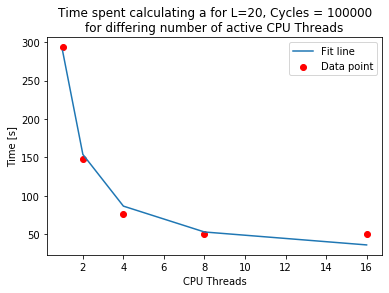
\includegraphics[scale=0.7]{timeThreads.png}
    \caption{Time spent calculating for a given number of threads with a best fit line}
    \label{fig3}
\end{figure} \newline
We see here that using multiple threads results in diminishing returns. This is very much in line with Amdahl's Law\cite{amdahl}, concerning the speedup/potential speed up for multi-threading a process. \newline
So yes, we are seeing speedup, but as we increase the number of threads we see diminishing returns. The sweet-spot for "the most value per thread" seems to be around 4-8 threads. \newline
It might've been possible to attain an even higher efficiency when multi-threading if I had instead used C++ for this project. Had it been possible I would've instead used the parallel python module, as my processor was locked at 66\% usage, even with all 16 available threads active. I suspect the primary culprit could be either the GIL (Global Interpreter Lock), or a part of processing power being set aside for Numpy, which I've read can happen. \newpage
\section{Conclusion}
In conclusion, we've shown and discussed at length different properties and curiosities with the Ising Model, and shown how it can be used to properly and accurate model a complex problem. We've done this by applying a Monte Carlo method onto it, the Metropolis algorithm, which in turn has allowed us to study it closer. Additionally we've inspected the behaviours of energy, magnetism, heat capacity and magnetic susceptibility for ferromagnetic materials, and we've used different results to further increase the complexity of our model to study a phase transition in detail, and although we could not derive a numerical $T_C$, we've discussed how it could be done given the proper data.
\bibliographystyle{plainurl}
\bibliography{citations.bib}
\newpage
\section*{Appendices}
\subsection*{Appendix A - Analytical Solutions of the $2\times 2$ lattice}
Following the theory described in Section [\ref{anal}], let us now examine the analytical solutions for a $2 \times 2$ lattice and solve them as a function of a temperature $T$.
\newline
Firstly, let us find the partition function:
\begin{equation*}
    Z = 2e^{8J\beta} + 2e^{-8J\beta} + 12 = 4\cosh{(8J\beta)} + 12
\end{equation*}
Knowing this, let us now calculate the rest.
\newline
Recall that the expectation values can also be calculate as:
\begin{equation*}
    \langle E \rangle = - \frac{\partial}{\partial \beta} \ln{Z}
\end{equation*}
which gives
\begin{equation*}
    \langle E \rangle = -8J \frac{\sinh{(8J\beta)}}{\cosh{(8J\beta)}+3}
\end{equation*}
Following the same principle, $\langle E^2 \rangle$ is:
\begin{equation*}
    \langle E \rangle = 64J^2 \frac{\cosh{(8J\beta)}}{\cosh{(8J\beta)}+3}
\end{equation*}
From Equation [\ref{m}], recall that $\langle M \rangle$ is found by summing over all possible states. To no surprise then, for a small lattice of $2 \times 2$, $\langle M \rangle$ becomes:
\begin{equation*}
    \langle M \rangle = \frac{1}{Z}(4e^{8J\beta} - 4e^{8J\beta} + 8 - 8) = 0
\end{equation*}
We can also find the square as:
\begin{equation*}
    \langle M^2 \rangle = 8 \frac{e^{8J\beta}+1}{\cosh(8J\beta)+3}
\end{equation*}
However, the absolute mean magnetization becomes:
\begin{equation*}
    \langle |M| \rangle = \frac{1}{Z}(4e^{8J\beta} + 4e^{8J\beta} + 16) = \frac{2e^{8J\beta} + 4}{\cosh{(8J\beta)} + 3}
\end{equation*}
We can then plug in these to find the variance, which we can then use to calculate $C_V$ and $\chi$ respectively.
\end{document}
